%\VignetteIndexEntry{An R Package for W-NOMINATE}
%\VignetteDepends{pscl}
%\VignetteKeywords{multivariate}
%\VignettePackage{wnominate}

\documentclass[12pt]{article}
\usepackage{Sweave}
\usepackage{amsmath}
\usepackage{amscd}

\begin{document}

\title{Using W-NOMINATE in R}
\author{James Lo}
\maketitle

\section{Introduction}

This package estimates Poole and Rosenthal W-NOMINATE scores from
roll call votes supplied though a \verb@rollcall@ object from package
\verb@pscl@.\footnote{Production of this package is supported by NSF Grant
SES-0611974.} The R version of W-NOMINATE computes ideal points using the same
Fortran code base as the previous \emph{wnom9707()} software.  It
improves upon the earlier software in three ways.  First, it is
now considerably easier to input new data for estimation, as the
current software no longer relies exclusively on the old
\emph{ORD} file format for data input.  Secondly, the software now
allows users to generate standard errors for their ideal point
estimates using a parametric bootstrap.  Finally, the
\verb@wnominate@ package includes a full suite of graphics
functions to analyze the results.

W-NOMINATE scores are based on the spatial model of voting.  Let
\textit{s} denote the number of policy dimensions, which are
indexed by \textit{k=1, \ldots, s}; let \textit{p} denote the
number of legislators (\textit{i=1,\ldots,p}); and \textit{q}
denote the number of roll call votes (\textit{j=1,\ldots,q}). Let
legislator \textit{i}'s ideal point be \textbf{$x_{i}$}, a vector
of length \textit{s}.  Each roll call vote is represented by
vectors of length \textit{s}, \textbf{$z_{jy}$} and
\textbf{$z_{jn}$}, where \textit{y} and \textit{n} stand for the
policy outcomes associated with Yea and Nay, respectively.

Legislator \textit{i}'s utility for outcome \textit{y} on roll
call \textit{j} is:

\begin{center}
{\Large
\begin{math}
 U_{ijy} = \beta
exp{[-\frac{\sum_{k=1}^{s}w^{2}_{k}d^{2}_{ijyk}}{2}]}
+\epsilon_{ijy}
\end{math}
}\\
\end{center}

The $d^{2}_{ijyk}$ term in the exponent is the Euclidean distance
between a legislator's ideal point $x_{i}$ and the Yea bill
location $z_{jyk}$; namely,


\begin{center}
{\Large
\begin{math}
d^{2}_{ijy}=\sum_{k=1}^{s}(x_{ik}-z_{jyk})^2
\end{math}
}
\end{center}

Weight $w$ and $\beta$ are estimated but set with initial values
of 0.5 and 15 respectively.  $\beta$ can be thought of as a
signal-to-noise ratio, where as $\beta$ increases in value, the
deterministic portion of the utility function overwhelms the
stochastic portion.  In multiple dimensions, $\beta$ is only
estimated for the first dimension and is thereafter kept constant.
For all other dimensions, the corresponding $w_{k}$ is estimated,
with the starting value of $w_{k}$ set at 0.5 each time.

In estimating the outcome points for each bill, W-NOMINATE estimates
the outcome points in terms of their midpoint and the distance between
them; namely,

\begin{center}
$z_{jy}=z_{mj}-d_{j}$ and $z_{jn}=z_{mj}+d_{j}$
\end{center}

where $z_{mj}$ is the midpoint and $d_{j}=\frac{z_{jy}-z_{jn}}{2}$.

\section{Usage Overview}

The \verb@wnominate@ package was designed for use in one of three
ways.  First, users can estimate ideal points from a set of
Congressional roll call votes stored in the traditional \emph{ORD}
file format.  Secondly, users can generate a vote matrix of their
own, and feed it directly into \verb@wnominate@ for analysis.
Finally, users can also generate test data with ideal points and
bill parameters arbitrarily specified as arguments by the user for
analysis with \verb@wnominate@. Each of these cases are supported
by a similar sequence of function calls, as shown in the diagrams
below:

\begin{flushleft}
$
\begin{CD}
\texttt{\emph{ORD} file}
   @>\texttt{readKH()}>>
   \texttt{\emph{rollcall} object}
   @>\texttt{wnominate()}>>
   \texttt{\emph{wnominate} object}
\end{CD}
$
$
\begin{CD}
   \texttt{Vote matrix}
   @>\texttt{rollcall()}>>
   \texttt{\emph{rollcall} object}
   @>\texttt{wnominate()}>>
   \texttt{\emph{wnominate} object}
\end{CD}
$
$
\begin{CD}
   \texttt{Arguments}
   @>\texttt{generateTestData()}>>
   \texttt{\emph{rollcall} object}
   @>\texttt{wnominate()}>>
   \texttt{\emph{wnominate} object}
\end{CD}
$
\end{flushleft}

Following generation of a \verb@wnominate@ object, the user then
analyzes the results using the \emph{plot} and \emph{summary} methods,
including:

\begin{itemize}
\item \textbf{plot.coords()}: Plots ideal points in one or two dimensions.
\item \textbf{plot.angles()}: Plots a histogram of cut lines.
\item \textbf{plot.cutlines()}: Plots a specified percentage of cutlines (a Coombs mesh).
\item \textbf{plot.skree()}: Plots a Skree plot with the first 20 eigenvalues.
\item \textbf{plot.nomObject()}: S3 method for a \verb@wnominate@ object
that combines the four plots described above.
\item \textbf{summary.nomObject()}: S3 method for a \verb@wnominate@ object
that summarizes the estimates.
\end{itemize}

Examples of each of the three cases described here are presented
in the following sections.

\section{W-NOMINATE with ORD files}

This is the use case that the majority of \verb@wnominate@ users
are likely to fall into.  Roll call votes in a fixed width format
\emph{ORD} format for all U.S. Congresses are stored online for
download at:

\begin{itemize}
\item \emph{http://www.voteview.com/} \item
\emph{http://www.polisci.ucla.edu/faculty/lewis/rollcall/} (latest Congress
only, updates votes in real time)
\end{itemize}

\verb@wnominate@ takes \verb@rollcall@ objects from Simon Jackman's
\verb@pscl@ package as input. The package includes a function,
\emph{readKH()}, that takes an \emph{ORD} file and automatically
transforms it into a \verb@rollcall@ object as desired. Refer to
the documentation in \verb@pscl@ for more detailed information on
\emph{readKH()} and \emph{rollcall()}.  Using the 90th Senate as
an example, we can download the file \emph{sen90kh.ord} and read
the data in R as follows:\\

\begin{Schunk}
\begin{Sinput}
> library(wnominate)
\end{Sinput}
\begin{Soutput}
pscl 0.75 	 2007-01-22 

## W-NOMINATE Ideal Point Package 
## Copyright 2006 - 2007 
## Keith Poole, Jeffrey Lewis, James Lo, and Royce Carroll
## Support provided by the U.S. National Science Foundation
## NSF Grant SES-0611974
\end{Soutput}
\begin{Sinput}
> data(sen90)
> sen90
\end{Sinput}
\begin{Soutput}
Source:		 C:/sen90kh.ord 
Number of Legislators:	 102 
Number of Votes:	 596 
Using the following codes to represent roll call votes:
Yea:		 1 2 3 
Nay:		 4 5 6 
Abstentions:	 7 8 9 
Not In Legislature:	 0 

Legislator-specific variables:
[1] "state"      "icpsrState" "cd"         "icpsrLegis" "party"     
[6] "partyCode" 
Detailed information available via summary function.
\end{Soutput}
\end{Schunk}

To make this example more interesting, suppose we were interested
in applying \emph{wnominate()} only to bills that pertained in some
way to agriculture.  Keith Poole and Howard Rosenthal's VOTEVIEW software allows us to
quickly determine which bills in the 90th Senate pertain to
agriculture.\footnote{VOTEVIEW for Windows can be downloaded at \emph{www.voteview.com}.}
Using this information, we create a vector of roll calls that we wish
to select, then select for them in the \verb@rollcall@ object.  In doing
so, we should also take care to update the variable in the \verb@rollcall@
object that counts the total number of bills, as follows:

\begin{Schunk}
\begin{Sinput}
> selector <- c(21, 22, 44, 45, 46, 47, 48, 49, 50, 53, 54, 55, 
+     56, 58, 59, 60, 61, 62, 65, 66, 67, 68, 69, 70, 71, 72, 73, 
+     74, 75, 77, 78, 80, 81, 82, 83, 84, 87, 99, 100, 101, 105, 
+     118, 119, 120, 128, 129, 130, 131, 132, 133, 134, 135, 141, 
+     142, 143, 144, 145, 147, 149, 151, 204, 209, 211, 218, 219, 
+     220, 221, 222, 223, 224, 225, 226, 227, 228, 229, 237, 238, 
+     239, 252, 253, 257, 260, 261, 265, 266, 268, 269, 270, 276, 
+     281, 290, 292, 293, 294, 295, 296, 302, 309, 319, 321, 322, 
+     323, 324, 325, 327, 330, 331, 332, 333, 335, 336, 337, 339, 
+     340, 346, 347, 357, 359, 367, 375, 377, 378, 379, 381, 384, 
+     386, 392, 393, 394, 405, 406, 410, 418, 427, 437, 442, 443, 
+     444, 448, 449, 450, 454, 455, 456, 459, 460, 461, 464, 465, 
+     467, 481, 487, 489, 490, 491, 492, 493, 495, 497, 501, 502, 
+     503, 504, 505, 506, 507, 514, 515, 522, 523, 529, 539, 540, 
+     541, 542, 543, 544, 546, 548, 549, 550, 551, 552, 553, 554, 
+     555, 556, 557, 558, 559, 560, 561, 562, 565, 566, 567, 568, 
+     569, 571, 584, 585, 586, 589, 590, 592, 593, 594, 595)
> sen90$m <- length(selector)
> sen90$votes <- sen90$votes[, selector]
\end{Sinput}
\end{Schunk}

\emph{wnominate()} takes a number of arguments described fully in
the documentation. Most of the arguments can (and probably should)
be left at their defaults, particularly when estimating ideal
points from U.S. Congresses.  The default options estimate ideal
points in two dimensions without standard errors, using the same
beta and weight parameters as described in the introduction. Votes
where the losing side has less than 2.5 per cent of the vote, and
legislators who vote less than 20 times are excluded from
analysis.

The most important argument that \emph{wnominate()} requires is a
set of legislators who have positive ideal points in each
dimension. This is the \emph{polarity} argument to \emph{wnominate()}.
In two dimensions, this might mean a fiscally conservative legislator
on the first dimension, and a socially conservative legislator on the
second dimension. Polarity can be set in a number of ways, such as a
vector of row indices (the recommended method), a
vector of names, or by any arbitrary column in the
\emph{legis.data} element of the \verb@rollcall@ object.  Here, we
use Senators Sparkman and Bartlett to set the polarity for the
estimation.  The names of the first 12 legislators are shown, and we
can see that Sparkman and Bartlett are the second and fifth
legislators respectively.

\begin{Schunk}
\begin{Sinput}
> rownames(sen90$votes)[1:12]
\end{Sinput}
\begin{Soutput}
 [1] "JOHNSON (D USA)"  "SPARKMAN (D AL)"  "HILL (D AL)"      "GRUENING (D AK)" 
 [5] "BARTLETT (D AK)"  "HAYDEN (D AZ)"    "FANNIN (R AZ)"    "FULBRIGHT (D AR)"
 [9] "MCCLELLAN (D AR)" "KUCHEL (R CA)"    "MURPHY (R CA)"    "DOMINICK (R CO)" 
\end{Soutput}
\begin{Sinput}
> result <- wnominate(sen90, polarity = c(2, 5))
\end{Sinput}
\begin{Soutput}
Preparing to run W-NOMINATE...

	Checking data...

		... 1 of 102 total members dropped.

		Votes dropped:
		... 36 of 208 total votes dropped.

	Running W-NOMINATE...

		Getting bill parameters...
		Getting legislator coordinates...
		Starting estimation of Beta...
		Getting bill parameters...
		Getting legislator coordinates...
		Starting estimation of Beta...
		Getting bill parameters...
		Getting legislator coordinates...
		Getting bill parameters...
		Getting legislator coordinates...
		Estimating weights...
		Getting bill parameters...
		Getting legislator coordinates...
		Estimating weights...
		Getting bill parameters...
		Getting legislator coordinates...


W-NOMINATE estimation completed successfully.
W-NOMINATE took 39.25 seconds to execute.
\end{Soutput}
\end{Schunk}

\verb@result@ now contains all of the information from the
W-NOMINATE estimation, the details of which are fully described in
the documentation for \emph{wnominate()}.
\verb@result$legislators@ contains all of the information from the
\verb@nom31.dat@ file from the old Fortran \emph{wnom9707()},
while \verb@result$rollcalls@ contains all of the information from
the old \verb@nom33.dat@ file.  The information can be browsed
using the \emph{fix()} command as follows (not run):\\

\noindent
> \emph{legisdata <- result\$legislators}\\
> \emph{fix(legisdata)}\\

For those interested in just the ideal points, a much better way
to do this is to use the \emph{summary()} function:

\begin{Schunk}
\begin{Sinput}
> summary(result)
\end{Sinput}
\begin{Soutput}
SUMMARY OF W-NOMINATE OBJECT
----------------------------

Number of Legislators:	  101 (1 legislators deleted)
Number of Votes:	  172 (36 votes deleted)
Number of Dimensions:	  2
Predicted Yeas:		  6551 of 7732 (84.7%) predictions correct
Predicted Nays:		  6418 of 7570 (84.8%) predictions correct
Correct Classifiction:	  79.77% 84.75%
APRE:			  0.365 0.521
GMP:			  0.652 0.708 


The first 10 legislator estimates are:
                 coord1D coord2D
JOHNSON (D USA)   -0.483  -0.142
SPARKMAN (D AL)    0.372   0.760
HILL (D AL)        0.625   0.719
GRUENING (D AK)   -0.706   0.709
BARTLETT (D AK)   -0.540   0.842
HAYDEN (D AZ)      0.156   0.876
FANNIN (R AZ)      0.803  -0.244
FULBRIGHT (D AR)   0.173   0.439
MCCLELLAN (D AR)   0.808   0.297
KUCHEL (R CA)     -0.199  -0.287
\end{Soutput}
\end{Schunk}

\verb@result@ can also be plotted, with a basic summary plot
achieved as follows as shown Figure 1:

\begin{figure}
\begin{center}
\begin{Schunk}
\begin{Sinput}
> plot(result)
\end{Sinput}
\begin{Soutput}
NULL
\end{Soutput}
\end{Schunk}
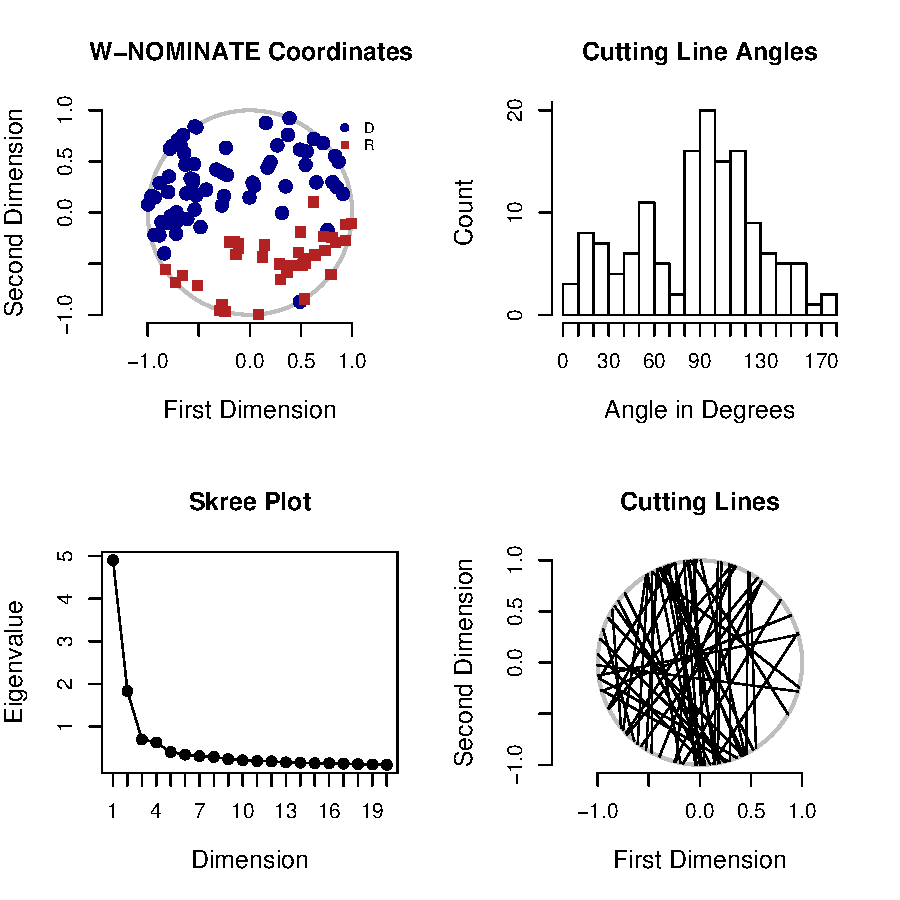
\includegraphics{wnominate-four}
\end{center}
\caption{Summary Plot of 90th Senate Agriculture Bill W-NOMINATE Scores}
\label{fig:one}
\end{figure}

This basic plot splits the window into 4 parts and calls
\emph{plot.coords()}, \emph{plot.angles()}, \emph{plot.skree()},
and \emph{plot.cutlines()} sequentially.  Each of these four
functions can be called individually.  In this example, the
coordinate plot on the top left plots each legislator with their
party affiliation. A unit circle is included to illustrate how
W-NOMINATE scores are constrained to lie within a unit circle.
Observe that with agriculture votes, party affiliation does not
appear to be a strong predictor on the first dimension, although
the second dimension is largely divided by party line.
The cutting angle histogram shows that most votes are well classified
by a single dimension (i.e. around 90$^\circ$), although there are a
number around 30$^\circ$ as well.  The Skree plot shows the first 20
eigenvalues, and the rapid decline after the second eigenvalue suggests
that a two-dimensional model describes the voting behavior of the 90th
Senate well.  The final plot shows 50 random cutlines, and can be
modified to show any desired number of cutlines as necessary.

Three things should be noted about the use of the \emph{plot()}
functions. First, the functions always plot the results from the
first two dimensions, but the dimensions used (as well as titles
and subheadings) can all be changed by the user if, for example,
they wish to plot dimensions 2 and 3 instead.  Secondly, plots of
one dimensional \verb@wnominate@ objects work somewhat differently
than in two dimensions
and are covered in the example in the final section.  Finally,
\emph{plot.coords()} can be modified to include cutlines from
whichever votes the user desires.  The cutline of the 14th 
agricultural vote (corresponding to the 58th actual vote)
from the 90th Senate with ideal points is plotted below in Figure
2, showing that the vote largely broke down along partisan
lines.

\begin{figure}
\begin{center}
\begin{Schunk}
\begin{Sinput}
> par(mfrow = c(1, 1))
> plot.coords(result, cutline = 14)
\end{Sinput}
\end{Schunk}
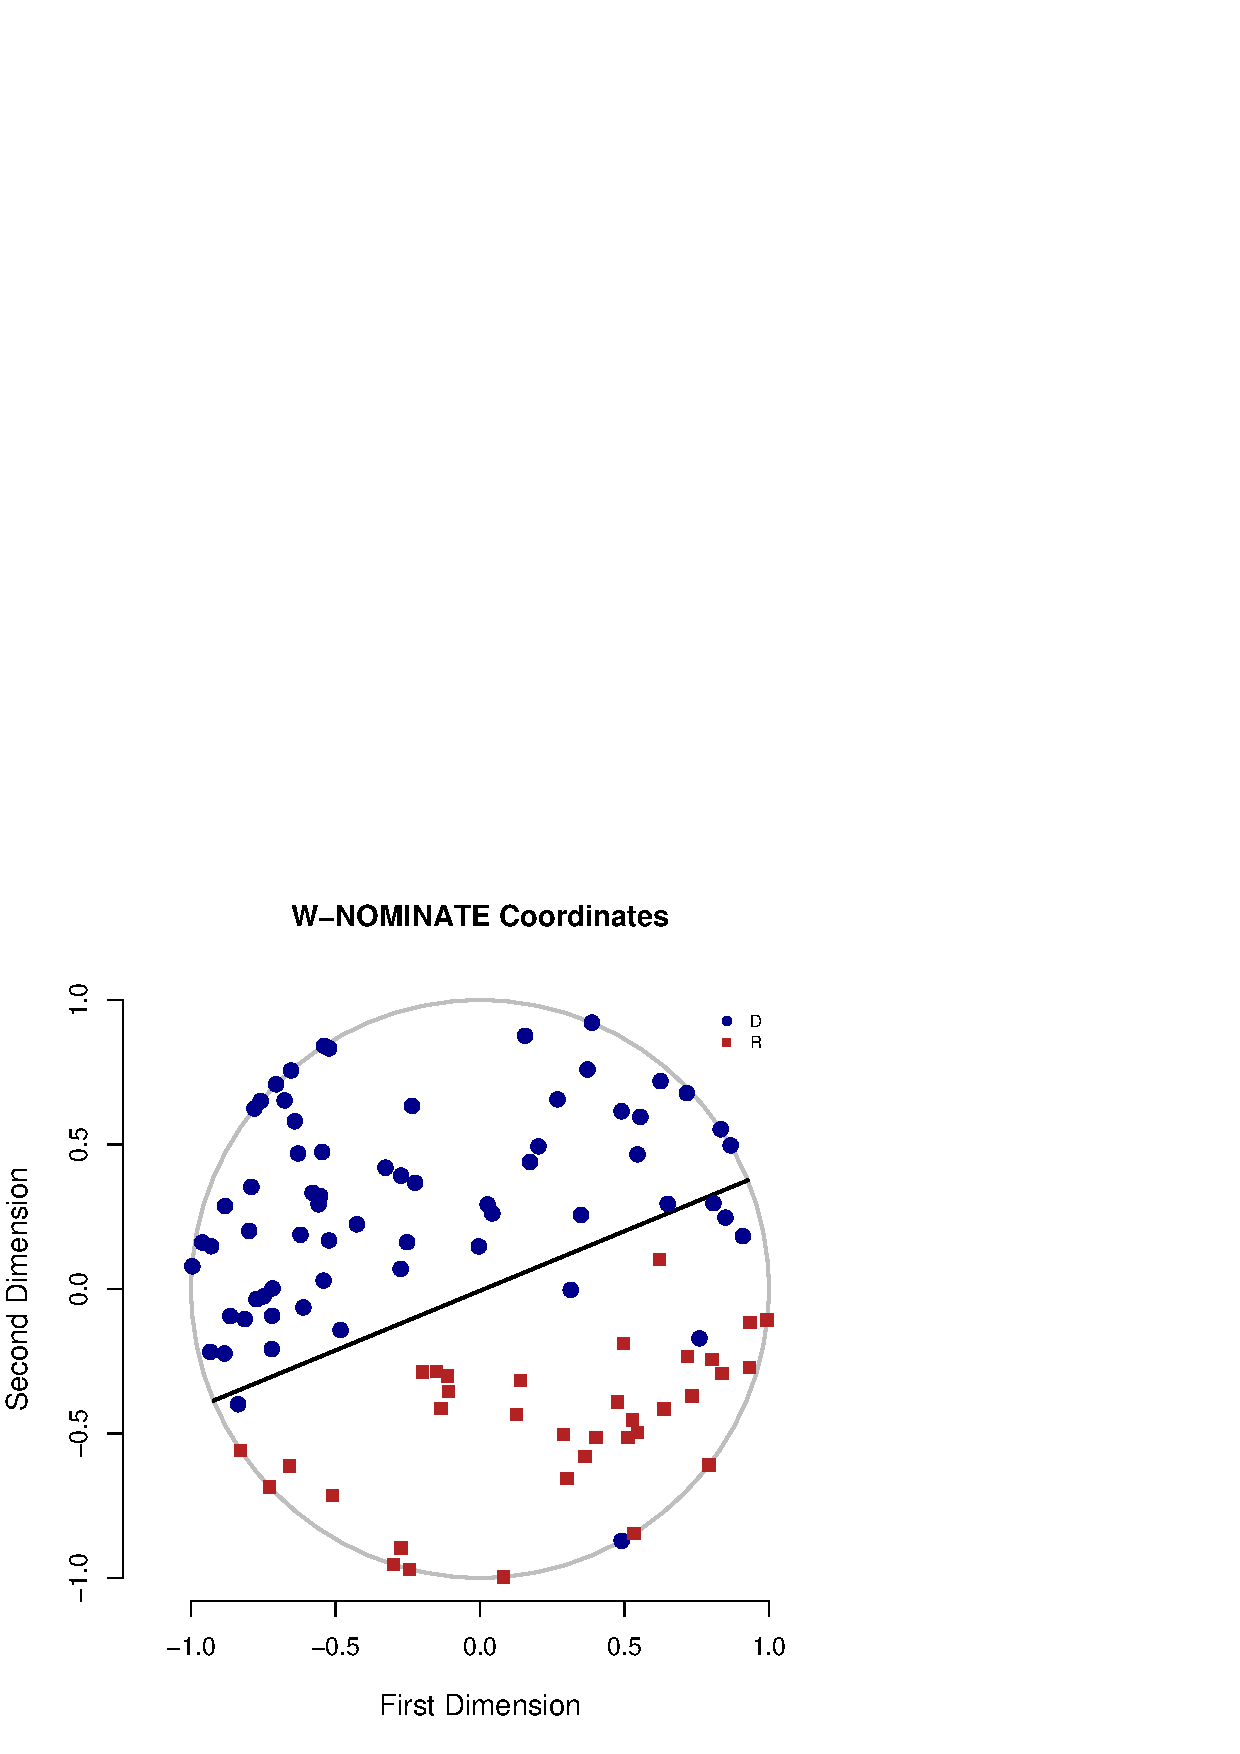
\includegraphics{wnominate-five}
\end{center}
\caption{90th Senate Agriculture Bill W-NOMINATE Scores with Cutline}
\label{fig:two}
\end{figure}

\section{W-NOMINATE with arbitrary vote matrix}

This section describes an example of W-NOMINATE being used for
roll call data not already in \emph{ORD} format.  The example here
is drawn from the first three sessions of the United Nations,
discussed further as Figure 5.8 in Keith Poole's \emph{Spatial
Models of Parliamentary Voting}.

To create a \verb@rollcall@ object for use with \emph{wnominate()},
one ideally should have three things:

\begin{itemize}
\item A matrix of votes from some source. The matrix should be
arranged as a \textit{legislators} x \textit{votes} matrix.  It
need not be in 1/6/9 or 1/0/NA format, but users must be able to
distinguish between Yea, Nay, and missing votes.

\item A vector of names for each member in the vote matrix.

\item OPTIONAL: A vector describing the party or party-like
memberships for the legislator.

\end{itemize}

The \verb@wnominate@ package includes all three of these items for
the United Nations, which can be loaded and browsed with the code 
shown below.  The data comes from Eric Voeten at George Washington University. 
In practice, one would prepare a roll call data set in a spreadsheet, like the
one available one \emph{www.voteview.com/UN.csv}, and read it into R using \emph{read.csv()}.
The csv file is also stored in this package and can be read using:\\

\noindent 
\emph{UN<-read.csv(``library/wnominate/data/UN.csv'',header=FALSE,strip.white=TRUE) }\\

%Does this work on Macs/Linux?

The line above reads the exact same data as what is stored in this
package as R data, which can be obtained using the following commands:

\begin{Schunk}
\begin{Sinput}
> rm(list = ls(all = TRUE))
> data(UN)
> UN <- as.matrix(UN)
> UN[1:5, 1:6]
\end{Sinput}
\begin{Soutput}
  V1              V2      V3  V4  V5  V6 
1 "United States" "Other" "1" "6" "6" "6"
2 "Canada"        "Other" "6" "6" "6" "6"
3 "Cuba"          "Other" "1" "6" "1" "1"
4 "Haiti"         "Other" "1" "6" "6" "9"
5 "Dominican Rep" "Other" "1" "6" "6" "7"
\end{Soutput}
\end{Schunk}

Observe that the first column are the names of the legislators
(in this case, countries), and the second column lists whether a
country is a ``Warsaw Pact'' country or ``Other'', which in this case can
be thought of as a `party' variable.  All other observations are votes.
Our objective here is to use this data to create a \verb@rollcall@ object
through the \emph{rollcall} function in \verb@pscl@.  The object can then
be used with \emph{wnominate()} and its plot/summary functions as in the
previous \emph{ORD} example.

To do this, we want to extract a vector of names (\emph{UNnames}) and party
memberships (\emph{party}), then delete them from the original matrix so we
have a matrix of nothing but votes. The \emph{party} variable must be rolled
into a matrix as well for inclusion in the \verb@rollcall@ object as
follows:

\begin{Schunk}
\begin{Sinput}
> UNnames <- UN[, 1]
> legData <- matrix(UN[, 2], length(UN[, 2]), 1)
> colnames(legData) <- "party"
> UN <- UN[, -c(1, 2)]
\end{Sinput}
\end{Schunk}

In this particular vote matrix, Yeas are numbered 1, 2, and 3, Nays are
4, 5, and 6, abstentions are 7, 8, and 9, and 0s are missing.  Other vote
matrices are likely different so the call to \emph{rollcall} will be slightly
different depending on how votes are coded.  Party identification is included
in the function call through \verb@legData@, and a \verb@rollcall@ object is
generated and applied to W-NOMINATE as follows.  The result is summarized below
and plotted in Figure 3:

\begin{Schunk}
\begin{Sinput}
> rc <- rollcall(UN, yea = c(1, 2, 3), nay = c(4, 5, 6), missing = c(7, 
+     8, 9), notInLegis = 0, legis.names = UNnames, legis.data = legData, 
+     desc = "UN Votes", source = "www.voteview.com")
> result <- wnominate(rc, polarity = c(1, 1))
\end{Sinput}
\begin{Soutput}
Preparing to run W-NOMINATE...

	Checking data...

		All members meet minimum vote requirements.

		Votes dropped:
		... 18 of 237 total votes dropped.

	Running W-NOMINATE...

		Getting bill parameters...
		Getting legislator coordinates...
		Starting estimation of Beta...
		Getting bill parameters...
		Getting legislator coordinates...
		Starting estimation of Beta...
		Getting bill parameters...
		Getting legislator coordinates...
		Getting bill parameters...
		Getting legislator coordinates...
		Estimating weights...
		Getting bill parameters...
		Getting legislator coordinates...
		Estimating weights...
		Getting bill parameters...
		Getting legislator coordinates...


W-NOMINATE estimation completed successfully.
W-NOMINATE took 34.83 seconds to execute.
\end{Soutput}
\end{Schunk}

\begin{Schunk}
\begin{Sinput}
> summary(result)
\end{Sinput}
\begin{Soutput}
SUMMARY OF W-NOMINATE OBJECT
----------------------------

Number of Legislators:	  59 (0 legislators deleted)
Number of Votes:	  219 (18 votes deleted)
Number of Dimensions:	  2
Predicted Yeas:		  4679 of 5039 (92.9%) predictions correct
Predicted Nays:		  4137 of 4488 (92.2%) predictions correct
Correct Classifiction:	  89.56% 92.54%
APRE:			  0.576 0.697
GMP:			  0.783 0.84 


The first 10 legislator estimates are:
              coord1D coord2D
United States   0.935   0.354
Canada          0.928   0.373
Cuba            0.517  -0.384
Haiti           0.357  -0.133
Dominican Rep   0.797  -0.215
Mexico          0.457   0.032
Guatemala       0.380   0.375
Honduras        0.587  -0.268
El Salvador     0.901  -0.433
Nicaragua       0.875  -0.250
\end{Soutput}
\end{Schunk}

\begin{figure}
\begin{center}
\begin{Schunk}
\begin{Sinput}
> plot(result)
\end{Sinput}
\begin{Soutput}
NULL
\end{Soutput}
\end{Schunk}
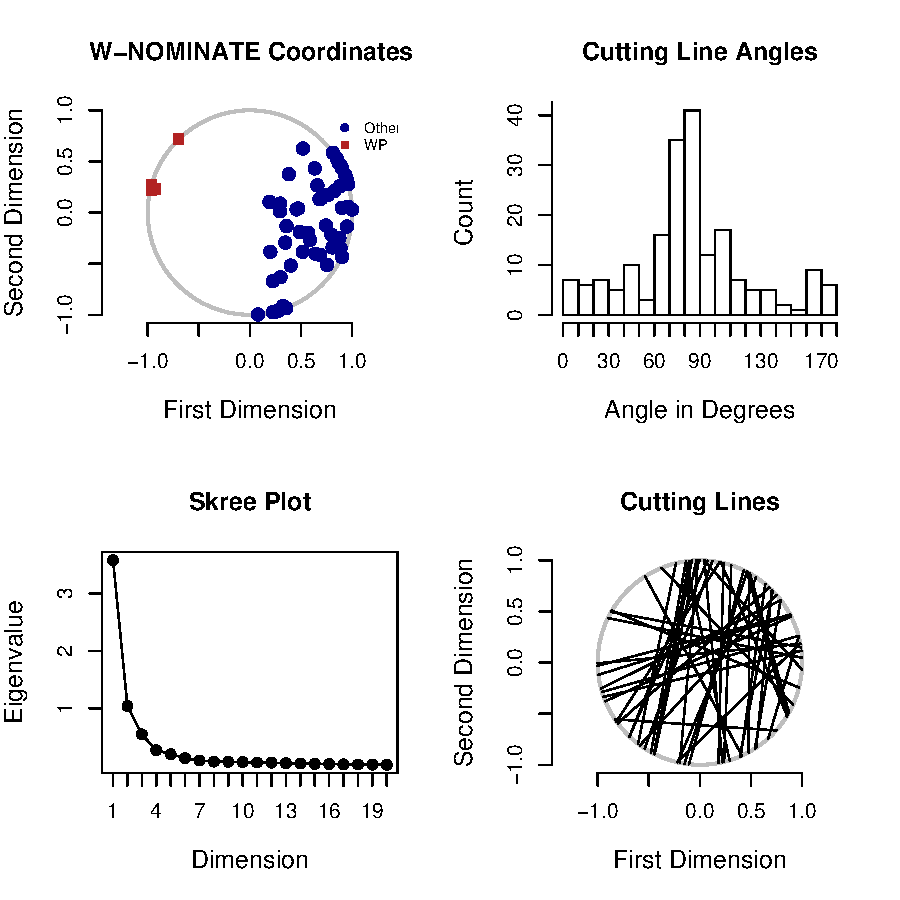
\includegraphics{wnominate-UN4}
\end{center}
\caption{Summary Plot of UN Data}
\label{fig:three}
\end{figure}

\section{W-NOMINATE with Test Data}

The W-NOMINATE package includes a test data generator that can be
used to generate arbitrary vote matrices.  These functions are
typically only used for testing purposes, and full documentation
of them is included with the package.  The two functions are:

\begin{itemize}
\item \emph{nomprob()}: A function that yields a matrix of
probabilities of a Yea vote.
\item \emph{generateTestData()}: A function that calls nomprob and
generates a \verb@rollcall@ object.
\end{itemize}

\textbf{nomprob()} takes a matrix of Yea and Nay locations, along with
a matrix of ideal points, and generates the vote probability matrix.
In this example, the Yea positions on 6 bills is set at 0.3, and the Nay
position is set at -0.2.  Bill parameters can be set in as many dimensions
as desired, but since the input matrices in this example have only one
column, the the bills are predominantly one-dimensional, as are the ideal
points.  For the ideal points, the first 5 legislators are set to have ideal
points of -0.2 while the last 5 are set to have ideal points of 0.2. This
setup leads to the last 5 legislators having a high probability of voting
Yea on all of the bills, as confirmed in the example, and vice versa. The
beta and weights can also be specified, and in this example we set them to
be the \emph{wnominate()} default values of 15 and 0.5. Both normal and
logistic link functions can be used to generate the probabilities,
although the default is to use normal probabilities.

\begin{Schunk}
\begin{Sinput}
> yp <- matrix(rep(0.3, 6), nrow = 6)
> np <- matrix(rep(-0.2, 6), nrow = 6)
> ideal <- matrix(c(rep(-0.2, 5), rep(0.2, 5)), nrow = 10)
> nomprob(yp, np, ideal, 15, 0.5)
\end{Sinput}
\begin{Soutput}
            [,1]       [,2]       [,3]       [,4]       [,5]       [,6]
 [1,] 0.03898851 0.03898851 0.03898851 0.03898851 0.03898851 0.03898851
 [2,] 0.03898851 0.03898851 0.03898851 0.03898851 0.03898851 0.03898851
 [3,] 0.03898851 0.03898851 0.03898851 0.03898851 0.03898851 0.03898851
 [4,] 0.03898851 0.03898851 0.03898851 0.03898851 0.03898851 0.03898851
 [5,] 0.03898851 0.03898851 0.03898851 0.03898851 0.03898851 0.03898851
 [6,] 0.85958172 0.85958172 0.85958172 0.85958172 0.85958172 0.85958172
 [7,] 0.85958172 0.85958172 0.85958172 0.85958172 0.85958172 0.85958172
 [8,] 0.85958172 0.85958172 0.85958172 0.85958172 0.85958172 0.85958172
 [9,] 0.85958172 0.85958172 0.85958172 0.85958172 0.85958172 0.85958172
[10,] 0.85958172 0.85958172 0.85958172 0.85958172 0.85958172 0.85958172
\end{Soutput}
\end{Schunk}

\textbf{generateTestData()} generates a full rollcall object using
\emph{nomprob()}, and in fact passes most of its arguments to it.  A totally
random set of parties and states are assigned to the legislators, so splits
by party and region are not substantively meaningful.  The function is set up
so that users need only specify the number of legislators and roll call votes
they wish to generate, and by default it generates a one dimensional model, as is shown here
in Figure 4:

\begin{Schunk}
\begin{Sinput}
> dat <- generateTestData(legislators = 100, rcVotes = 1000)
> result <- wnominate(dat, polarity = 1, dims = 1)
\end{Sinput}
\begin{Soutput}
Preparing to run W-NOMINATE...

	Checking data...

		All members meet minimum vote requirements.

		All votes meet minimum lopsidedness requirement.

	Running W-NOMINATE...

		Getting bill parameters...
		Getting legislator coordinates...
		Starting estimation of Beta...
		Getting bill parameters...
		Getting legislator coordinates...
		Starting estimation of Beta...
		Getting bill parameters...
		Getting legislator coordinates...


W-NOMINATE estimation completed successfully.
W-NOMINATE took 152.81 seconds to execute.
\end{Soutput}
\begin{Sinput}
> summary(result)
\end{Sinput}
\begin{Soutput}
SUMMARY OF W-NOMINATE OBJECT
----------------------------

Number of Legislators:	  100 (0 legislators deleted)
Number of Votes:	  1000 (0 votes deleted)
Number of Dimensions:	  1
Predicted Yeas:		  48664 of 53110 (91.6%) predictions correct
Predicted Nays:		  41632 of 46890 (88.8%) predictions correct
Correct Classifiction:	  90.3%
APRE:			  0.78
GMP:			  0.808 


The first 10 legislator estimates are:
             coord1D se1D
Legislator1    0.848    0
Legislator2   -0.494    0
Legislator3    0.244    0
Legislator4    0.679    0
Legislator5    0.249    0
Legislator6    0.330    0
Legislator7   -0.286    0
Legislator8    0.511    0
Legislator9   -1.000    0
Legislator10  -0.084    0
\end{Soutput}
\end{Schunk}

\begin{figure}
\begin{center}
\begin{Schunk}
\begin{Sinput}
> plot(result)
\end{Sinput}
\end{Schunk}
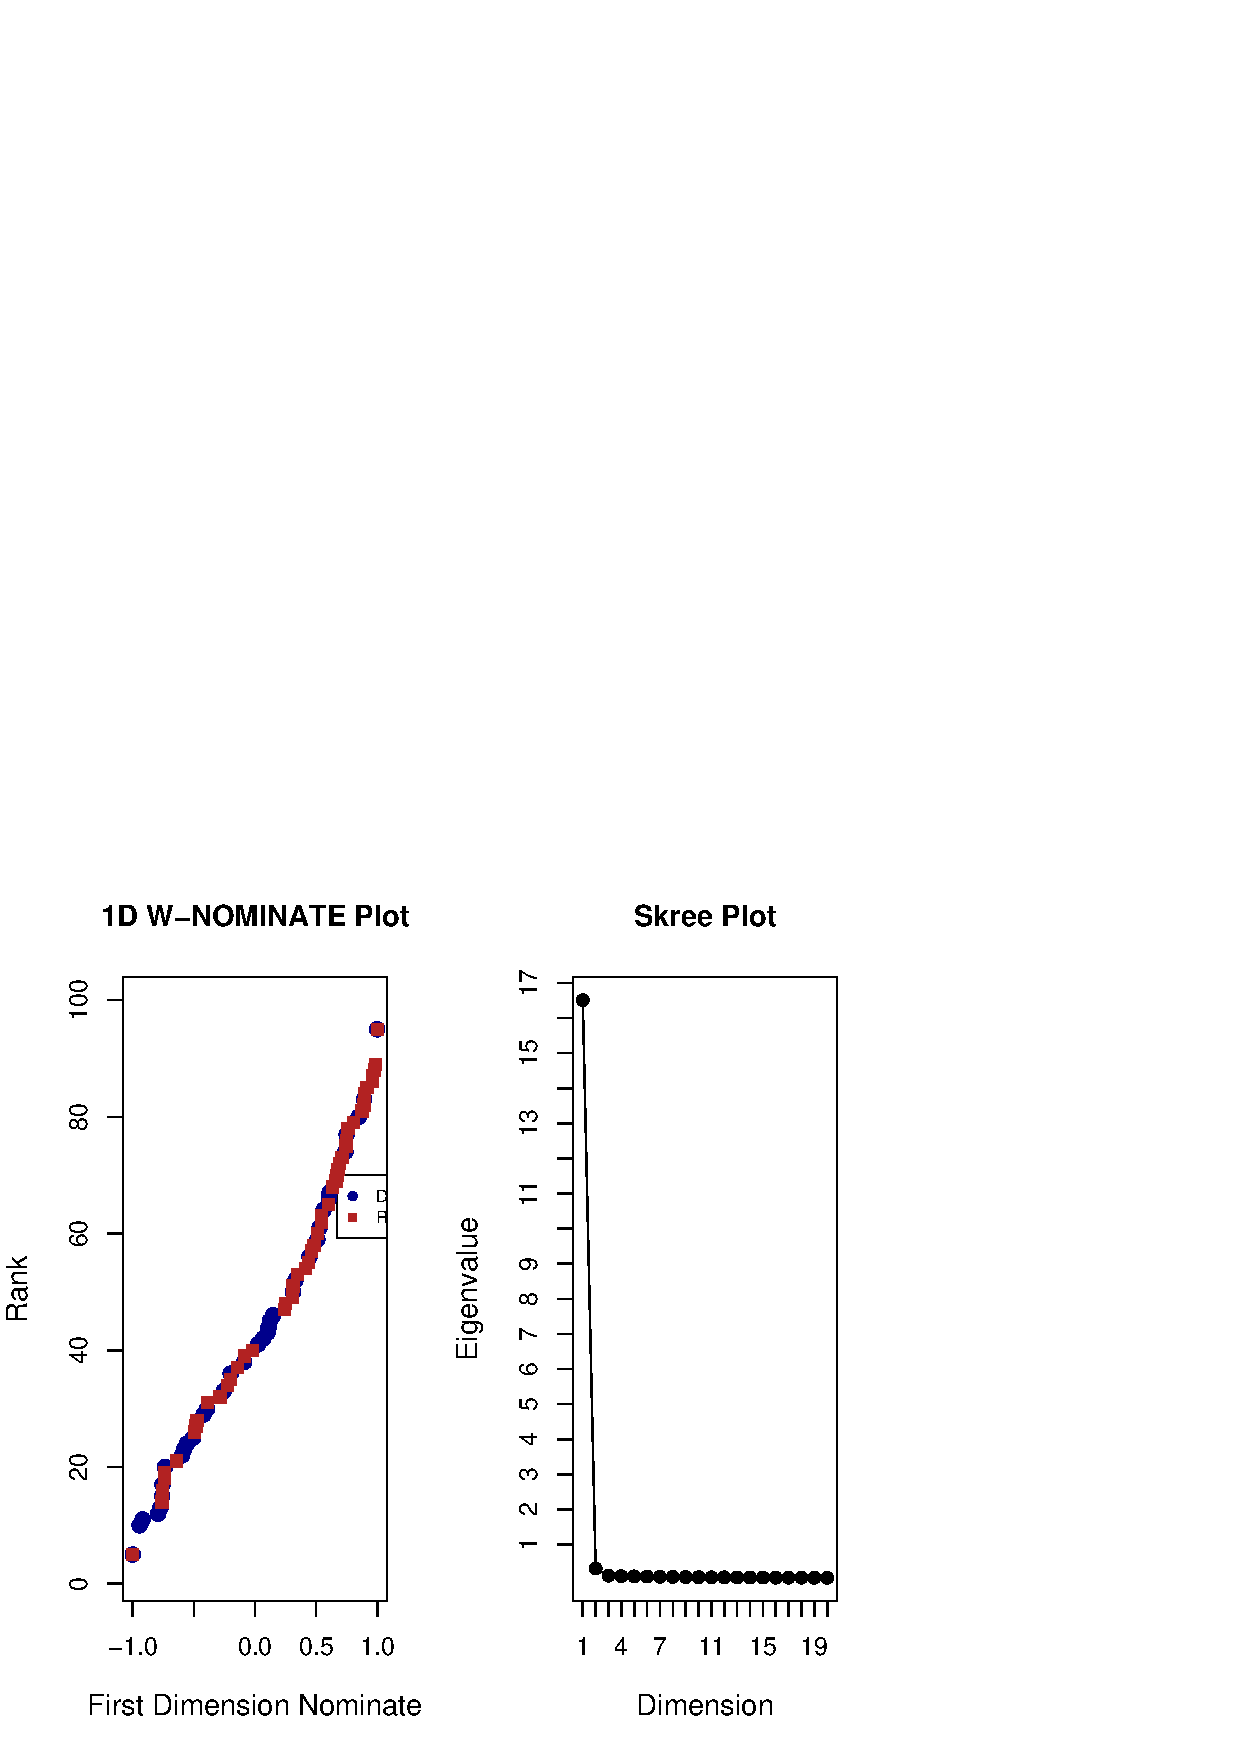
\includegraphics{wnominate-random3}
\end{center}
\caption{Summary Plot of Randomly Generated Data}
\label{fig:four}
\end{figure}

Note that the one dimensional plot differs considerably from the previous two dimensional
plots, since only a coordinate plot and a Skree plot are shown.  This is because in one
dimension, all cutlines are angled at 90$^\circ$, so there is no need to plot either the
cutlines or a histogram of cutline angles.  Also, the plot appears to be compressed,
so users need to expand the image manually by using their mouse and dragging along
the corner of the plot to expand it.  The Skree plot confirms that a single dimension captures
the voting patterns accurately, as seen by the flatness of the curve from the second
dimension on.

\newpage
\begin{thebibliography}{3}

\bibitem{Bootstrap} Lewis, Jeffrey B. and Poole, Keith (2004)
``Measuring Bias and Uncertainty in Ideal Point Estimates via the Parametric Bootstrap.''
\emph{Political Analysis} 12(2): 105-127.

\bibitem{Congress} Poole, Keith (2005)
\emph{Spatial Models of Parliamentary Voting.}
Cambridge: Cambridge University Press.

\bibitem{Congress} Poole, Keith and Howard Rosenthal (1997)
\emph{Congress: A Political-Economic History of Roll Call Voting.}
New York: Oxford University Press.

\end{thebibliography}

\end{document}
